\section{PROCEDIMIENTO} 

\begin{itemize}
\subsection{Ejercicio 1: Envios}
	\subsubsection{Enunciado}

		\item El siguiente diagrama E / R simplificado describe el envío de mercancías. Los lotes pertenecientes a ciertos grupos se
envían a ciertos destinos en varios países a través de diferentes modos de transporte. Un cierto centro de costos es responsable de cada envío. La dimensión de tiempo consiste en mes y año.

	\begin{center}
	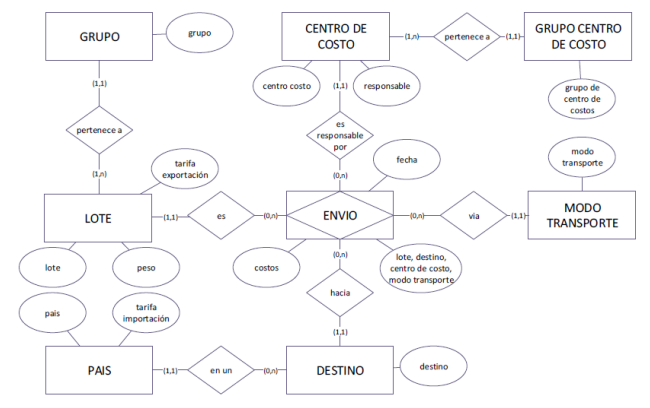
\includegraphics[width=14cm]{./Imagenes/ejercicio1}
	\end{center}

     \subsubsection{Modelo Dimensional }
	\begin{center}
	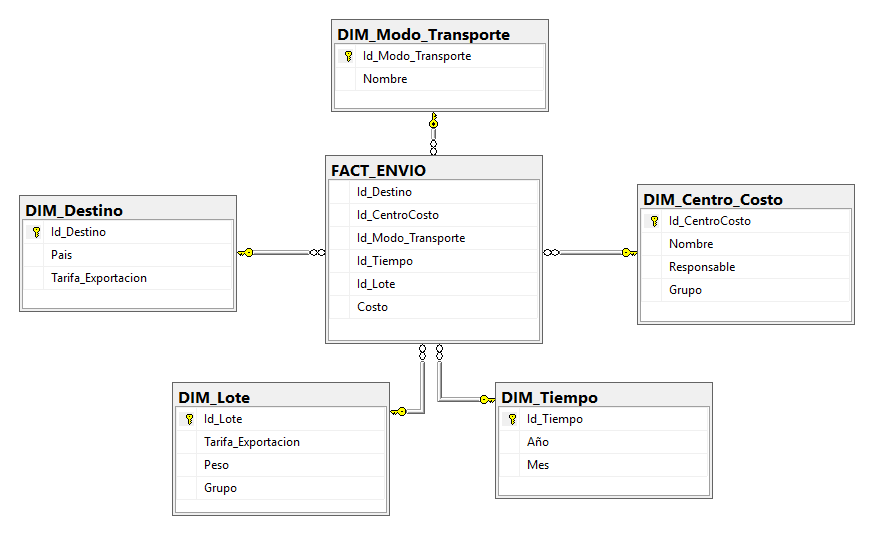
\includegraphics[width=14cm]{./Imagenes/ejercicio1_dimensional}
	\end{center}
   \subsubsection{Diagrama Físico }
	
	\begin{center}
	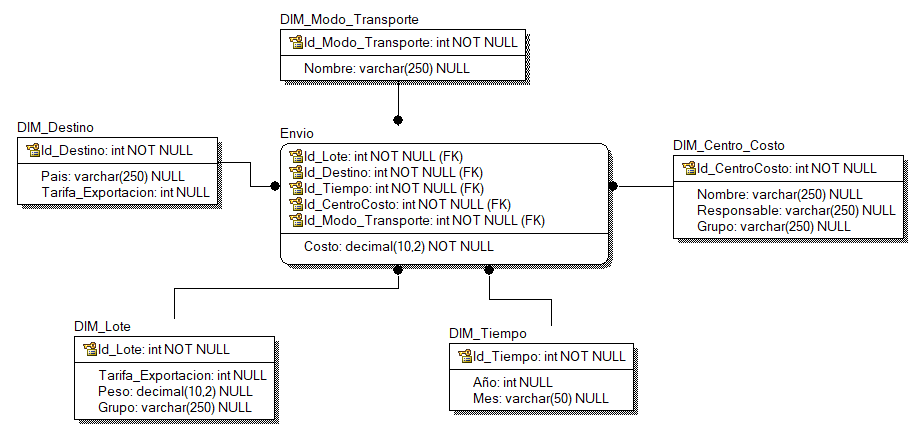
\includegraphics[width=14cm]{./Imagenes/ejercicio1_fisico}
	\end{center}

 \subsubsection{Script }
\begin{center}
	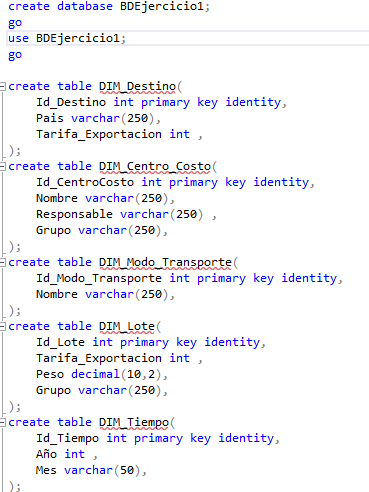
\includegraphics[width=8cm]{./Imagenes/ej1_script1}
	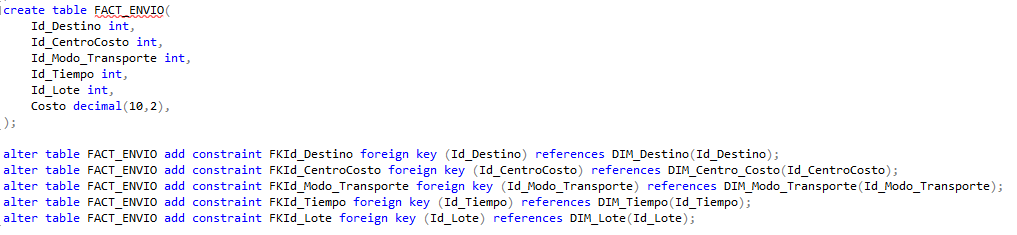
\includegraphics[width=14cm]{./Imagenes/ej1_script2}
	\end{center}


\subsection{Ejercicio 2: : Reservas de Viaje}

\subsubsection{Enunciado}

		\item En este esquema de E / R, un cliente (que es de cierto tipo) reserva un viaje en una agencia de viajes. La agencia de viajes trabaja para un determinado operador turístico. El viaje va a un destino determinado que pertenece a un país determinado.
La dimensión de tiempo consiste en mes, trimestre y año.

	\begin{center}
	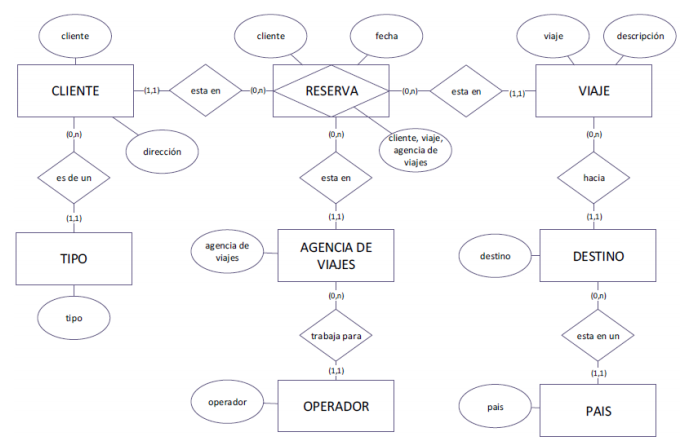
\includegraphics[width=14cm]{./Imagenes/ejercicio2}
	\end{center}

     \subsubsection{Modelo Dimensional }
	\begin{center}
	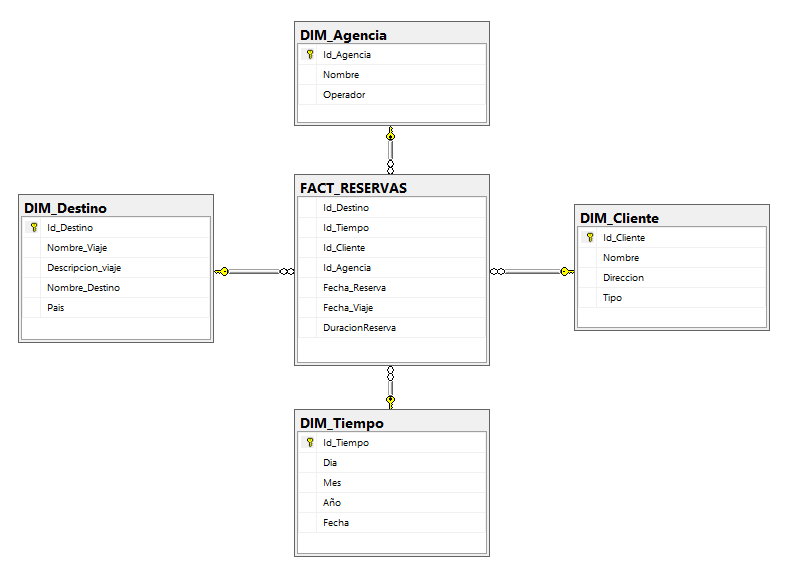
\includegraphics[width=14cm]{./Imagenes/ejercicio2_dimensional}
	\end{center}
   \subsubsection{Diagrama Físico }
	
	\begin{center}
	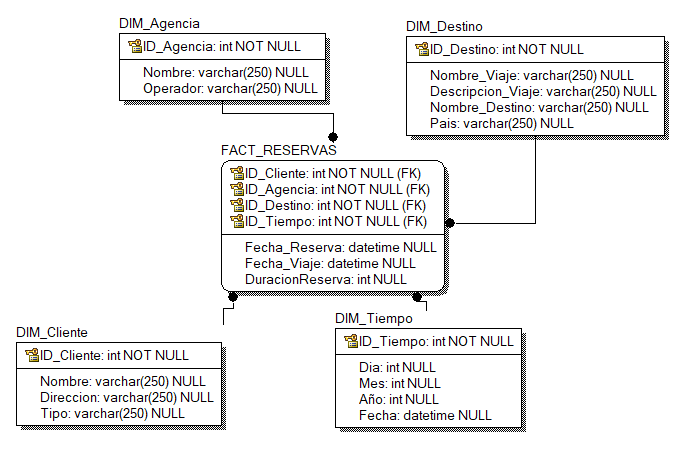
\includegraphics[width=14cm]{./Imagenes/ejercicio2_fisico}
	\end{center}

 \subsubsection{Script }
\begin{center}
	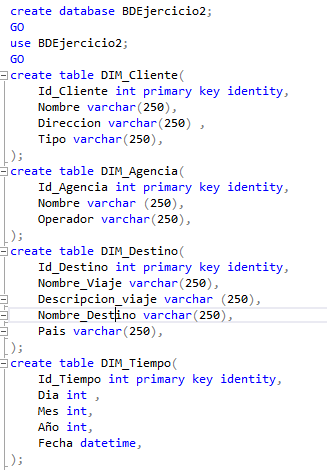
\includegraphics[width=8cm]{./Imagenes/ej2_script1}
	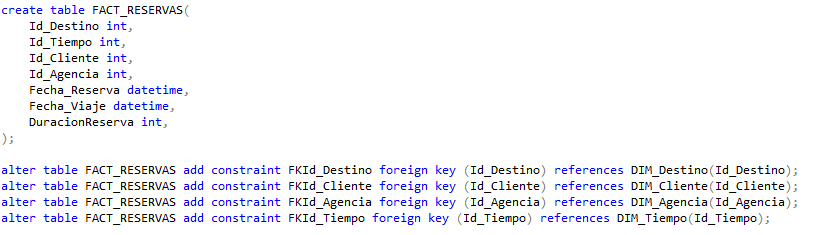
\includegraphics[width=14cm]{./Imagenes/ej2_script2}
	\end{center}

\subsection{Ejercicio 3: Gestión de proyectos}

\subsubsection{Enunciado}

		\item Este esquema E / R simplificado muestra un caso gestión del proyecto. El proyecto para un cliente se divide en varios paquetes de trabajo y siempre una persona es responsable de completar la tarea. Se cuida en un lugar determinado.
La dimensión de tiempo consiste de día, mes y año.

	\begin{center}
	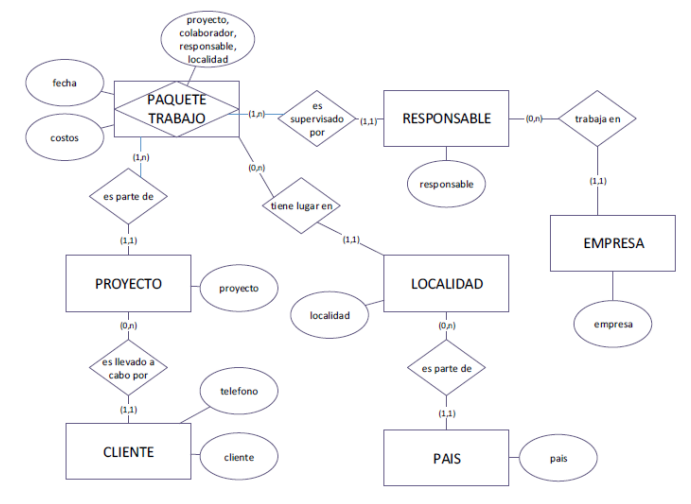
\includegraphics[width=14cm]{./Imagenes/ejercicio3}
	\end{center}

     \subsubsection{Modelo Dimensional }
	\begin{center}
	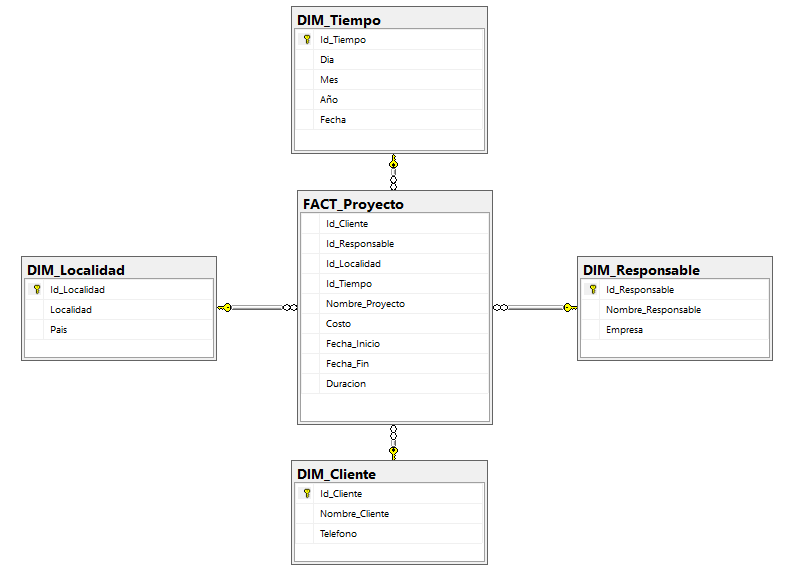
\includegraphics[width=14cm]{./Imagenes/ejercicio3_dimensional}
	\end{center}
   \subsubsection{Diagrama Físico }
	
	\begin{center}
	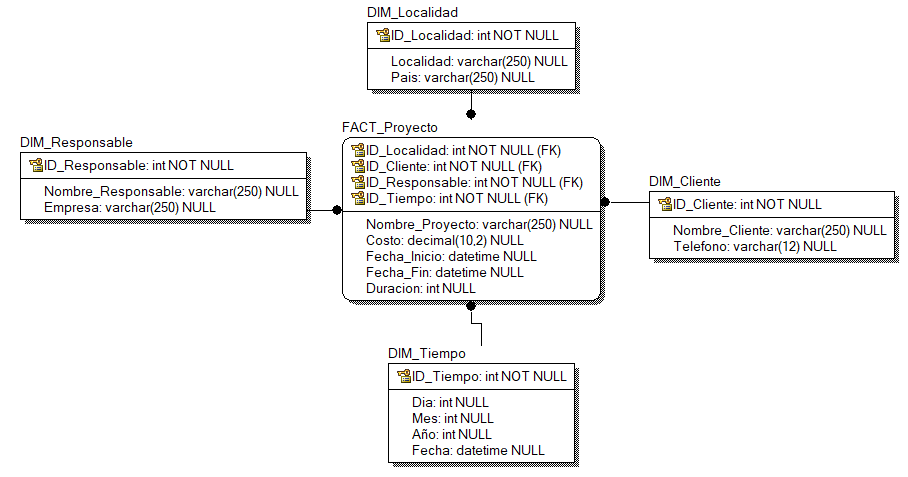
\includegraphics[width=14cm]{./Imagenes/ejercicio3_fisico}
	\end{center}

 \subsubsection{Script }
\begin{center}
	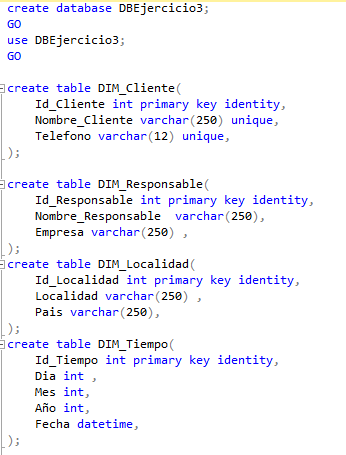
\includegraphics[width=8cm]{./Imagenes/ej3_script1}
	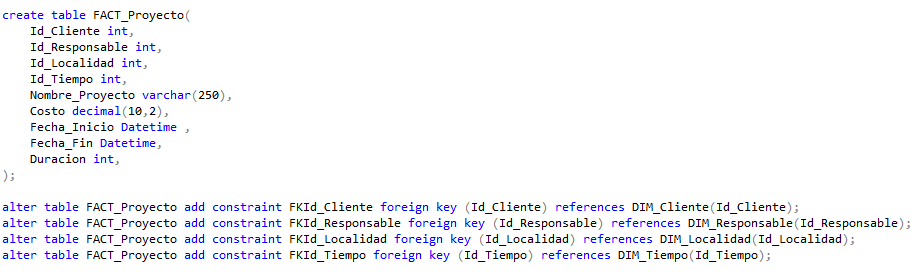
\includegraphics[width=14cm]{./Imagenes/ej3_script2}
	\end{center}

\end{itemize}
		